\scanpage{86}

\inserted{Of course, one could \unsure{derive} \unsure{analogues} from it \deleted{\illegible{1}} at will}
\inserted{the Theorem 1, 1°, hypothesis b)}

\deleted{Of course, \unsure{by virtue of} the \unsure{indicated|analogous} inequality,}
\[
\deleted{(\unsure{7|4|11})\qquad \sum\varphi(-\alpha_1,\unsure{\mathord{-}},-\alpha_n)\leq\sum\varphi(\unsure{-}\beta_1,\unsure{\mathord{-}},\unsure{-}\beta_n)}
\]

\uline{Remark 1} Let us note, \deleted{\unsure{moreover|however}}, that if two sequences $(\alpha_i)_{i\leq n},(\beta_i)_{i\leq n}$ satisfy the general conditions of the \deleted{lemma}\inserted{theorem 1, 1°} \inserted{$(\alpha_1\geq\mathord{-}\geq\alpha_n,\ \alpha_1+\unsure{\mathord{-}}\alpha_M\leq\beta_1+\mathord{\cdot}\,\mathord{\cdot}+\beta_M\ \deleted{\unsure{and}}\ 1\leq M\leq n$} then \deleted{it is so for the \unsure{same sequences} $(\alpha_i)_{i\leq p},(\beta_i)_{i\leq p}$ for every $1\leq p\leq n$, \unsure{(provided of course that} $\sum_1^p\alpha_i=\sum_1^p\beta_i$), therefore one can apply to them the \unsure{formula} of the lemma, and \unsure{one obtains} for \unsure{example} $\varphi(\alpha_1,\unsure{\mathord{-}},\alpha_p)$ which one obtains by replacing $\alpha_{p+1},\unsure{\mathord{-}},\alpha_n$ and $\beta_{p+1},\unsure{\mathord{-}},\beta_n$ by}

\inserted{sequences with $k$ elements} $(\alpha_i)_{i\leq k}$ and $(\beta_i)_{i\leq k}$ \inserted{satisfy the analogous conditions} \deleted{for every}\inserted{for every} $1\leq k\leq n$. One can therefore apply the same lemma to these sequences, and one finds \deleted{\unsure{therefore}}\inserted{for example} that \deleted{\unsure{(at the cost of} \illegible{2} \unsure{the lemma}} \inserted{if $\varphi$ is a convex function} increasing in \uline{$k$} arguments, one also has $\varphi(\alpha_1,\mathord{\cdot}\,\mathord{-}\alpha_k)\leq\varphi(\beta_1,\mathord{-}\,\mathord{-},\beta_k)$. The analogous remark holds for the \deleted{corollary 1 of the lemma}\inserted{conditions of theorem 1, 2°}.

\reversemarginpar
\margin{\uline{Remark 2} If one assumes $(\alpha_i)$ $(\beta_i)$ \unsure{as} in hypothesis a, and if $f(\alpha_1\mathord{-}\alpha_n)\leq f(\beta_1\mathord{-}\beta_n)$ for \deleted{\unsure{every}} $f$ \unsure{such|such} \unsure{$\in$|that} \ldots{} then one has $\sum_1^m\alpha_i\leq\sum_1^m\beta_i$ (obviously, this amounting to $\sup_H\sum_{i\in H}\alpha_i$, \deleted{\unsure{where}} $H$ with \deleted{\unsure{at most}} \inserted{$m$ elements})}
\margin{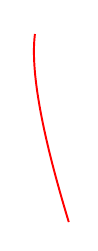
\begin{tikzpicture}[x=.01cm,y=-.01cm,baseline]\draw[red,line width=.7pt] (12,8) .. controls (4,70) and (35,181) .. (55,247);\end{tikzpicture}}
\normalmarginpar

\deleted{\uline{Applications \unsure{new of the inequality|and examples of convexity} \unsure{to|of} corollary 1.}}

Let us now give an interesting case of functions $f$ satisfying the conditions of the \deleted{corollary 1}\inserted{theorem 1, 2°}. \deleted{\unsure{which is}}

If \uline{\deleted{\unsure{$f(\rho_1$}} $f(\rho_1,\mathord{-}\rho_n)$ is a convex increasing function of the \inserted{the set of} arguments $\rho_i>0$, then $f(e^{t_1},\mathord{-}e^{t_n})$ is \deleted{\unsure{convex}}}\inserted{a} convex function of \deleted{\unsure{each of the arguments}} $(t_i)\in R^{n}$. Since \deleted{the convex function \unsure{will be the one which is}} \inserted{$f$ will be} an upper envelope of \deleted{\unsure{linear}}\inserted{linear} affine functions \inserted{$\sum a_i x_i+\underset{\text{\unsure{arbitrary}}}{b}$, $a_i\geq0$ (!)}, $f(e^{t_1},\mathord{-}e^{t_n})$ will be an upper envelope \deleted{and that every convex function} of functions $\sum a_i e^{t_i}+b$, which are convex (for \deleted{\unsure{if}} the functions $e^{t_i}$ are convex, and the $a_i$ positive), therefore it will itself be convex.

In particular, \deleted{if $f$ by a \deleted{function}\inserted{\unsure{norm}} of \unsure{Schatten}} \unsure{let us call|appl.ons}, \uline{Schatten \unsure{norm|norms}} on $R^n$ any \uline{norm} $N(x)=N(x_1,\mathord{-}x_n)$ which is symmetric, such that $N(x_1,\mathord{-}x_n)=N(|x_1|,\mathord{-}\,\mathord{-}|x_n|)$, \deleted{and which is an increasing function of each of the arguments for} \inserted{$x_1\geq0,\mathord{-}\,\mathord{-}x_n\geq0$}, \deleted{\unsure{and thereby is therefore} \illegible{2}} \inserted{normalized by $N(e_1)=1$.}

\reversemarginpar
\margin{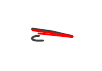
\begin{tikzpicture}[x=1cm,y=1cm,baseline]\draw[black!75,line width=1pt,line cap=round] (.02,.11)--(.27,.075)--(.53,.015);\draw[black!75,line width=.7pt,line cap=round] (.11,.025).. controls (-.015,.025) and (-.025,-.055)..(.16,-.035);\draw[red,line width=.65pt,line cap=round] (.025,.095)--(.50,.025);\draw[red,line width=.65pt,line cap=round] (.10,.055)--(.53,.01);\end{tikzpicture}}
\margin{(Then one proves that $N$ is an increasing function \deleted{\unsure{of the arguments}} \unsure{$(x_i)$|$(\alpha_i)$} in \unsure{the orthant} of positive elements ((for the unit ball, being stable under multiplication by a function $(\lambda_i)$ with $|\lambda_i|=1$ for \deleted{every} $i$, will be so for \deleted{\unsure{every}} function bounded by $1$ in modulus).}
\margin{87}
\normalmarginpar
